\chapter{Un dígito hecho de Sol -- I}
\label{sec:digito-solar-i}

\lettrine[ante=\raisebox{-1.5ex}{\large ---},lines=2]{C}{ada uno de}
los dígitos que indicarán la hora estarán formados por rayos de Sol
---arrancó Antonia, ofreciendo a Cecilia la figura \ref{fig:digitos}.

\begin{figure}[ht]
  \centering
\centerline{
  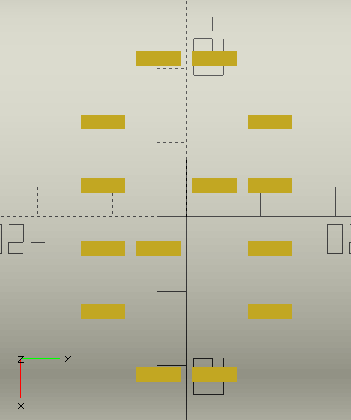
\includegraphics[height=.25\textwidth]{imagenes/cero}
  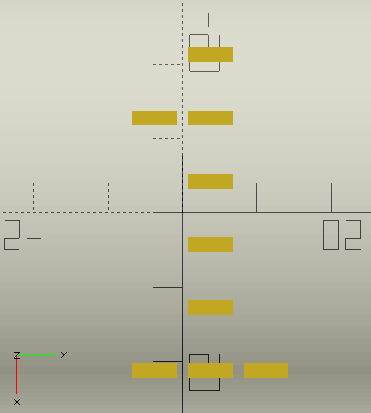
\includegraphics[height=.25\textwidth]{imagenes/uno}
  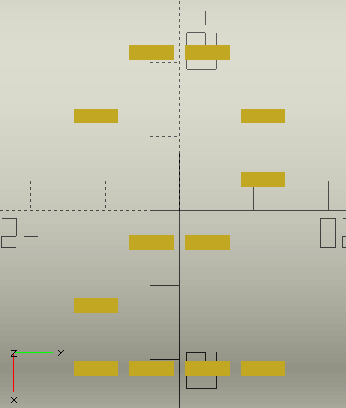
\includegraphics[height=.25\textwidth]{imagenes/dos}
}
\centerline{
  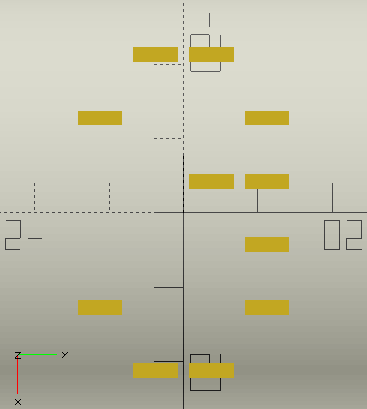
\includegraphics[height=.25\textwidth]{imagenes/tres}
  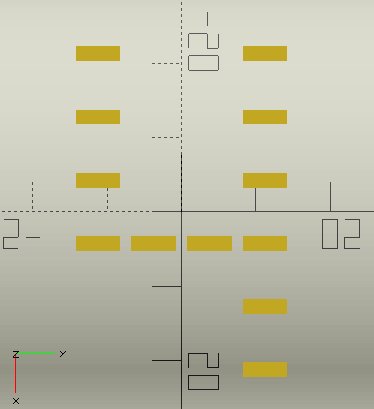
\includegraphics[height=.25\textwidth]{imagenes/cuatro}
  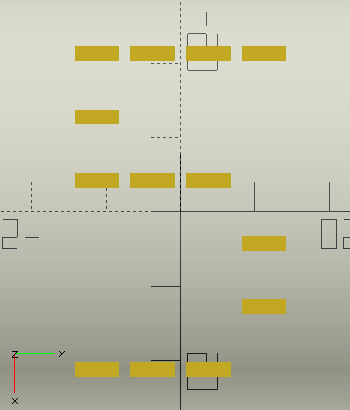
\includegraphics[height=.25\textwidth]{imagenes/cinco}
}
\centerline{
  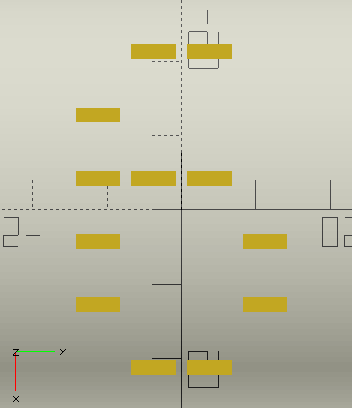
\includegraphics[height=.25\textwidth]{imagenes/seis}
  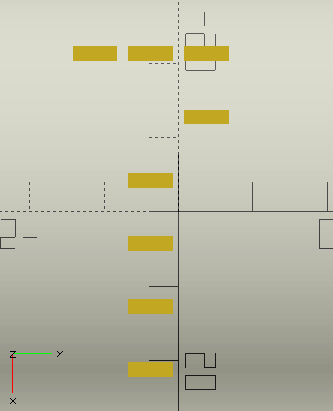
\includegraphics[height=.25\textwidth]{imagenes/siete}
  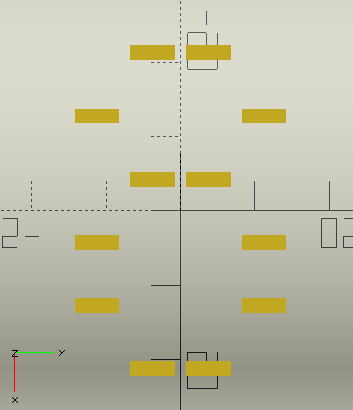
\includegraphics[height=.25\textwidth]{imagenes/ocho}
  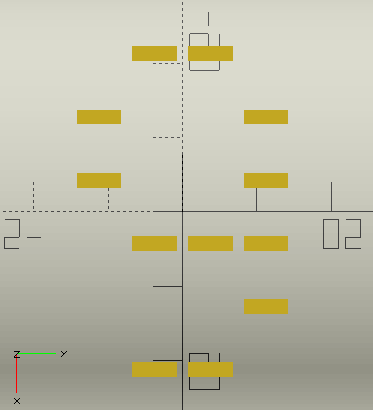
\includegraphics[height=.25\textwidth]{imagenes/nueve}
}  
  \caption{Dígitos hechos de rayos de Sol.}
  \label{fig:digitos}
\end{figure}

---¡Qué buenos diseños! ¿Los hiciste vos? ---preguntó Cecilia.


---No ---reconoció Antonia sin dificultad---. La disposición visual la
copié inescrupulosamente del modelo que me inspiró en general:
\url{https://www.thingiverse.com/thing:1068443}.

---¡Ah! Sos pilla... ---Cecilia sonrió con malicia.

---Fue sólo el aspecto visual ---Antonia se refugió en una
actitud defensiva---. La lógica y el texto los reconstruí
  yo sola.

Cecilia miró unos instantes a su amiga detenidamente; no sabía si
hacerle una pregunta. Finalmente la soltó:

---Antonia... ¿Por qué rehiciste un modelo que ya fue resuelto por
otra persona? ¿No te bastaba bajarlo e imprimirlo?

Antonia devolvió a Cecilia la mirada:

---¿Por qué estás haciendo este curso? ---replicó---. ¿Por qué
llegaste a la página \thepage{} de este manualcito?

Las dos amigas se miraron en silencio. Cecilia comprendió que pocas
cosas se comparaban con resolver, por una misma, un problema difícil y
con un resultado final de aspecto hermoso. Y el reloj de Sol digital
combinaba ambas cualidades a la perfección.

---Como habrás notado ---retomó Antonia---, todos los dígitos se basan
en un mismo patrón de seis filas y cuatro columnas de pixeles. La
diferencia entre los dígitos reside en los pixeles que están
`encendidos' o `apagados'; aunque sería mejor decir `abiertos' o
`cerrados', dado que cada uno representa un agujero en el semicilindro
del reloj.

---El `1' parece contar con tres columnas, solamente ---ob\-ser\-vó
Cecilia.

---La cuarta columna está, sólo que formada por pixeles `cerrados'
---aclaró Antonia. A Cecilia le pareció un poco artificial. <<¿Y por
qué no pensar, entonces, que está formado por 17 filas y 48 columnas,
la mayoría de ellas `cerradas'?>> ---pensó, pero la dejó continuar.

\begin{figure}[t]
  \centering
  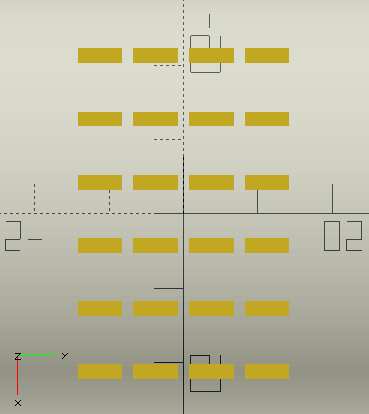
\includegraphics[width=.35\textwidth]{imagenes/matriz}
  \caption{Matriz de pixeles que formarán cada dígito.}
  \label{fig:matriz}
\end{figure}

---Para aclarar ideas, vamos a ver todos los rayos `encendidos'
---dijo Antonia señalando la figura \ref{fig:matriz}, mientras
prosiguía con el lento tono que presagiaba una de sus largas
explicaciones---. Cada dígito, entonces, se formará dejando abiertos o
cerrados los pixeles adecuados. Pero antes de ver cómo elegir cada
uno, creo que es mejor que resolvamos el problema de ubicar cada rayo
en una disposición ordenada y prolija de filas y columnas.

Cecilia puso cara de inteligente:

---¿Usamos la transformación \lstinline!translate!?

---Sí, más vale; pero la pregunta es \emph{¿cómo?} ---Antonia pareció
no haber captado la ironía---. A mí me sirve empezar haciendo
dibujitos encima ---agregó, realizando la figura
\ref{fig:matriz-anotada-2}.

\begin{figure}[ht]
  \centering
  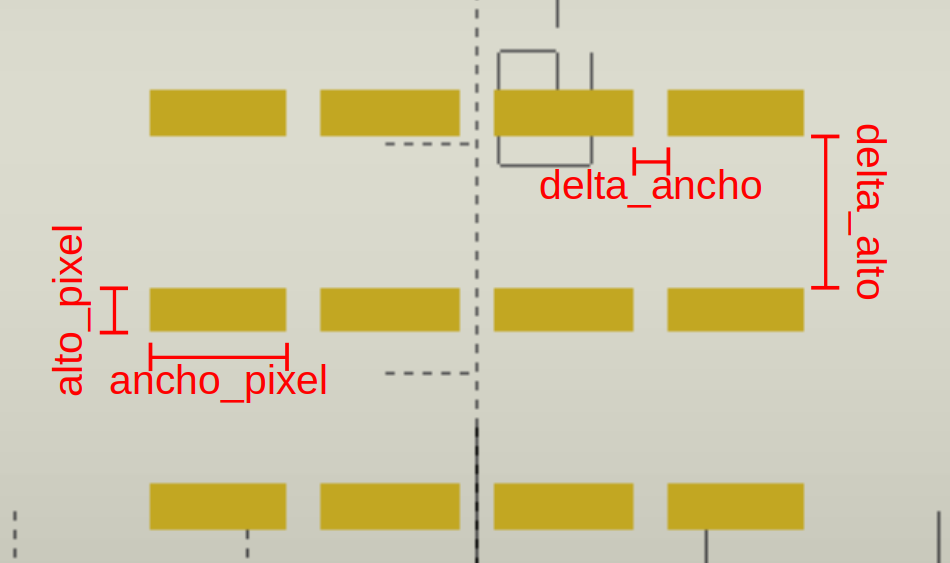
\includegraphics[width=.55\textwidth]{imagenes/matriz-anotada-2}
  \caption{Antonia anota la matriz con el fin de ubicar cada pixel.}
  \label{fig:matriz-anotada-2}
\end{figure}
  


\guillemotright Para poder distribuir correctamente los pixeles,
debemos ponernos de acuerdo no sólo en el tamaño de cada pixel
(expresado en nuestros conocidos \texttt{ancho\_pixel} y
\texttt{alto\_pixel}) sino también en la separación entre pixeles: se
me ocurrió llamarlos \texttt{delta\_ancho} y
\texttt{delta\_alto}... básicamente porque sí.

Cecilia no tuvo nada que objetar.

---Ahora tenemos que poder distinguir a cada pixel de los
demás. Ponerles un `nombre', digamos. Se me ocurrió que hacerlo en
referencia a la fila y columna que ocupan en el arreglo no puede ser
la peor forma ---dijo Antonia.

\begin{figure}[ht]
  \centering
  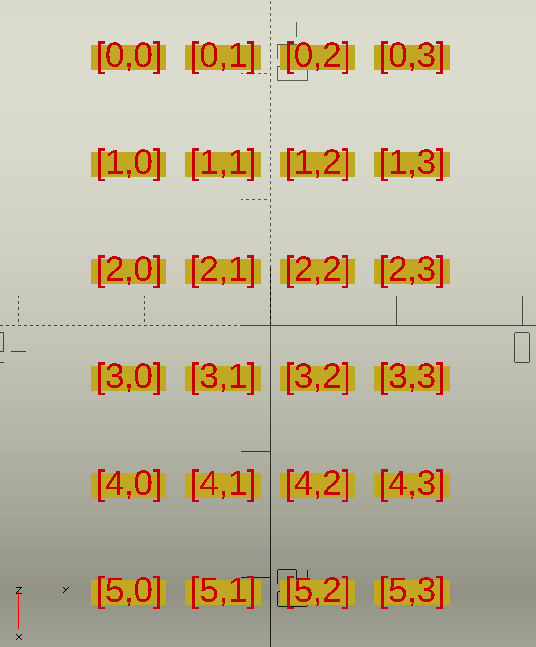
\includegraphics[width=.45\textwidth]{imagenes/matriz-anotada-coordenadas}
  \caption{Antonia nombra cada pixel con las coordenadas enteras de su
    matriz.}
  \label{fig:matriz-anotada-coordenadas}
\end{figure}
  


\guillemotright Así, el primer pixel será el de la fila 0 y columna 0,
etc. Como comentamos en el capítulo \ref{sec:vectores}, es usual
referirse a las posiciones dentro de un arreglo rectangular empezando
por 0 ---recordó Antonia, y prosiguió---: Ahora, lo más difícil:
ubicar la posición en \coord{X} e \coord{Y} de cada pixel conociendo
su fila y columna, tomando en cuenta los valores de
\texttt{ancho\_pixel}, \texttt{alto\_pixel}, \texttt{delta\_ancho} y
\texttt{delta\_alto}.

%Antonia escribió un poco más antes de seguir con su monólogo:

\guillemotright Para ir paso a paso, me parece mejor ubicar como
origen de coordenadas el centro del pixel \texttt{[0,0]}. Sí, ya sé
---se adelantó---; nosotras queremos que sea el centro del arreglo el
que esté en el origen de coordenadas; pero creo que es más fácil
comenzar a pensarlo así.

Cecilia no se sentía con muchas ganas de contradecir a Antonia,
básicamente porque aún no sabía exactamente adónde se dirigía en ese
camino que ya le parecía demasiado largo.

---Muy bien, Cecilia; ya hablé mucho ---Antonia miró a su amiga con
los ojos apenas entornados y con un brillo que, una vez más, parecía
una súplica---. Ahora tendríamos que ser capaces de calcular el valor
de \coord{X} e \coord{Y} para cualquier pixel: digamos, por ejemplo,
el \texttt{[3,2]}.



\begin{figure}[ht]
  \centering
  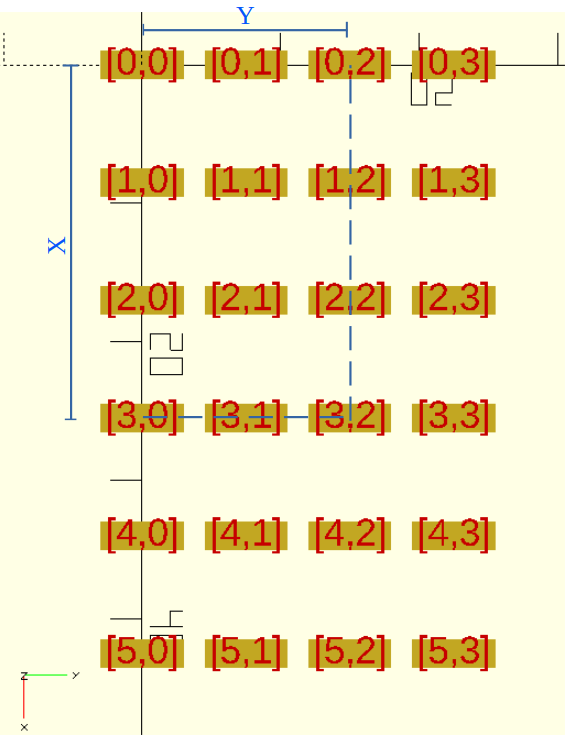
\includegraphics[width=.42\textwidth]{imagenes/matriz-coordenadas-1}
  \caption{Antonia desafía a Cecilia a encontrar las coordenadas
    \coord{X} e \coord{Y} de cada pixel; en particular, del
    \texttt{[3,2]}.}
  \label{fig:matriz-coordenadas-1}
\end{figure}

Antonia hizo silencio, y Cecilia supo que aquel plural era, como otras
veces, bien singular.

---¿Me dejás hacer unos dibujitos? ---preguntó Cecilia mientras tomaba
para sí el teclado.

\begin{figure}[ht]
  \centering
  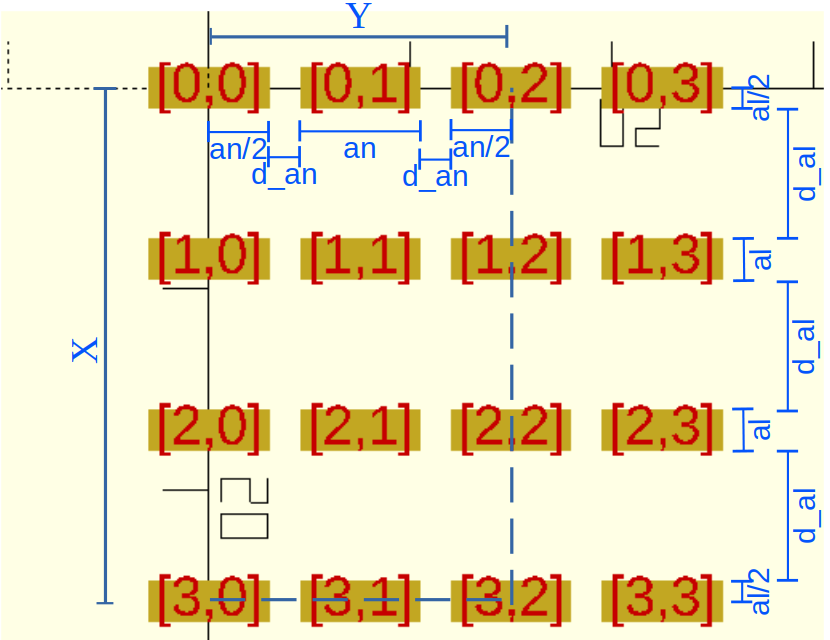
\includegraphics[width=.6\textwidth]{imagenes/matriz-coordenadas-4}
  \caption{Cecilia procura expresar las coordenadas \coord{X} e
    \coord{Y} de cada pixel, comenzando por el \texttt{[3,2]}.}
  \label{fig:matriz-coordenadas-4}
\end{figure}

\guillemotright ¡Uf! Me costó... ---reconoció mientras se reclinaba
pesadamente contra el respaldo de la silla y contemplaba la flamante
figura \ref{fig:matriz-coordenadas-4}---. Como no me entraba en el
dibujo, tuve que usar abreviaturas: \texttt{an} es
\texttt{ancho\_pixel}, \texttt{d\_an} es \texttt{delta\_ancho}... en
fin, creo que lo demás se entiende.

Antonia asintió con entusiasmo.

---Por lo que veo ---Cecilia continuó---, la coordenada \coord{Y} del
pixel \texttt{[3,2]} es igual a
$\frac{\text{an}}{2}+\text{d\_an}+\text{an}+\text{d\_an}+\frac{\text{an}}{2}=2\times
\text{an} + 2\times\text{d\_an}=2\times(\text{an}+\text{d\_an})$. Por
otra parte, la coordenada \coord{X} parece ser igual a... ---Cecilia
masculló apenas los pasos intermedios---:
$3\times(\text{al}+\text{d\_al})$.

Antonia, con una amplia sonrisa de satusfacción, tomó la palabra y el
teclado:

---Pasemos en limpio, entonces:

\[
  \text{Para el pixel }[3,2]: \left\{
    \begin{aligned}
      X&=3\times(\text{al}+\text{d\_al})\\
      Y&=2\times(\text{an}+\text{d\_an})
    \end{aligned}
  \right.
\]

Cecilia contemplaba las ecuaciones y el grafico. No pasó mucho tiempo
hasta que encontró el patrón subyacente:

---¡Claro! ---exclamó exultante---. La coordenada \coord{X} del pixel
\texttt{[i,j]} es $i$ veces $(\text{al}+\text{d\_al})$ , mientras que
la coordenada \coord{Y}, análogamente, es $j$ veces
$(\text{an}+\text{d\_an})$.\footnote{Sería bueno demostrar
  fehacientemente un aserto tan general (Nota del
  Editor).}$^,$\footnote{¿No tenés nada mejor que hacer?  (Nota de
  Cecilia, Antonia y Luis).}

Antonia confirmó la conclusión de Cecilia con indisimulada alegría:

---Vamos a dejarlo bien patente ---propuso.


\begin{equation}
  \text{Para el pixel }[i,j]: \left\{
    \begin{aligned}
      X&=i\times(\text{al}+\text{d\_al})\\
      Y&=j\times(\text{an}+\text{d\_an})
    \end{aligned}
  \right.\label{eq:coordenadas-matriz}
\end{equation}

\guillemotright Creo que es hora de darle a tantas vueltas y rodeos la
forma de un texto para \openscad{}, ¿no te parece? ---invitó Antonia,
cediéndole el teclado con gesto ceremonioso.

Cecilia lo tomó con decisión, aún no del todo segura de lo que iba a
escribir, pero con entusiasmo y la confianza de que las teclas
\keystroke{Supr} y \keystroke{$\Longleftarrow$} le serían fieles. Tras
mucho escribir, borrar y consultar con las ecuaciones, obtuvo lo
siguiente:

%    \begin{center}
 % \begin{minipage}[]{1\textwidth}%\vspace{0pt}
    \begin{lstlisting}
alto_pixel  = 2;
ancho_pixel = 6;      
delta_alto  = 6.5;
delta_ancho = 1.5;

module digito(alfa){
  for(i=[0:5],j=[0:3]){
   x=i*(alto_pixel+delta_alto);
   y=j*(ancho_pixel+delta_ancho);
   translate([x,y,0])
    rayo_de_sol(alfa);
  }
}

digito(alfa=90);
    \end{lstlisting}
%  \end{minipage}\hfill

    \begin{figure}[ht]
      \centering
    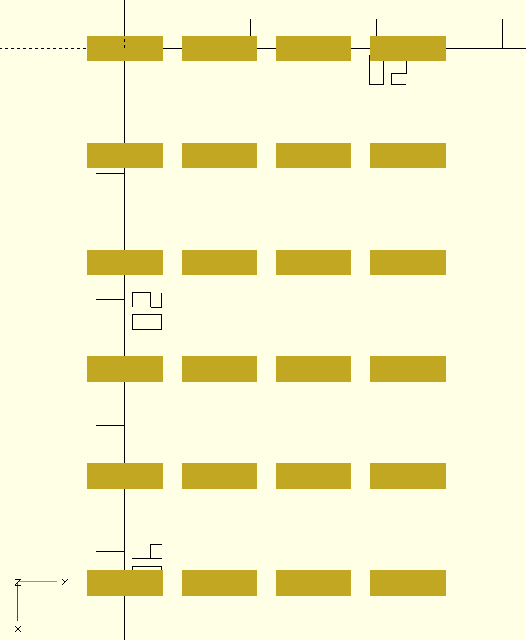
\includegraphics[width=.4\textwidth]{imagenes/matriz-completa}  
    \caption{Cecilia logra producir una matriz completa de pixeles
      encendidos.}
      \label{fig:matriz-completa}
    \end{figure}
    



    Cecilia se sentía tan feliz contemplando el resultado plasmado en
    la figura \ref{fig:matriz-completa} que pensaba que podría releer
    su texto hasta que el Sol se
    apagara. % Sabía que el objetivo del presente
    % capítulo era encontrar una manera de crear una ordenación
    % rectangular de pixeles, para luego elegir cuales abrir y cuales
    % cerrar; por esa razón, no puso mucho cuidado a la hora de nombrar
    % su módulo: \texttt{arreglo\_completo} era suficientemente bueno
    % para un módulo auxiliar, que sería borrado tras comprobarse la
    % efectividad del método.

    Dentro del módulo creaba un doble bucle: las variables \texttt{i}
    y \texttt{j} recorrían los valores de 0 a 5 y de 0 a 3,
    respectivamente, a fin de abarcar todas las filas y columnas.

    Luego, en las líneas 8 y 9 calculaba las coordenadas \coord{X} e
    \coord{Y} de cada pixel, aplicando las ecuaciones
    \ref{eq:coordenadas-matriz}.

    Por último, en las líneas 10 y 11 creaba para cada pixel un rayo
    de Sol trasladado a las coordenadas recién calculadas.

    ---Parece mentira que además funcione, ¿no? ---Antonia interrumpió
    los pensamientos de Cecilia---. A mí me pasa lo mismo: una cosa es
    \emph{saber} que un algoritmo debe funcionar, y otra muy distinta
    es \emph{comprobar} que efectivamente funciona. Es... hermoso.

    Cecilia estaba de acuerdo de todo corazón. Pero Antonia se
    reservaba una objeción:

    ---Fijate la posición del arreglo completo: te quedó centrado en
    su pixel \texttt{[0,0]}, no en su centro.
    
    Cecilia se mordió el labio inferior; la ansiada versión final del
    texto siempre parecía alejarse un poco más.

    ---Es cierto --admitió---; pero parece sencillo de resolver: no
    hay más que trasladar todo una cierta distancia en \coord{X} e
    \coord{Y}... a ver... ---y Cecilia, en breves instantes, pudo
    ofrecer su nueva solución:

    \begin{lstlisting}
module digito(alfa){
  translate([-2.5*(alto_pixel+delta_alto),
             -1.5*(ancho_pixel+delta_ancho),
             0])
   for(i=[0:5],j=[0:3]){
    x=i*(alto_pixel+delta_alto);
    y=j*(ancho_pixel+delta_ancho);
    translate([x,y,0])
     rayo_de_sol(alfa);
   } 
}

digito(alfa=90);
    \end{lstlisting}

  
  \begin{figure}[ht]
    \centering
    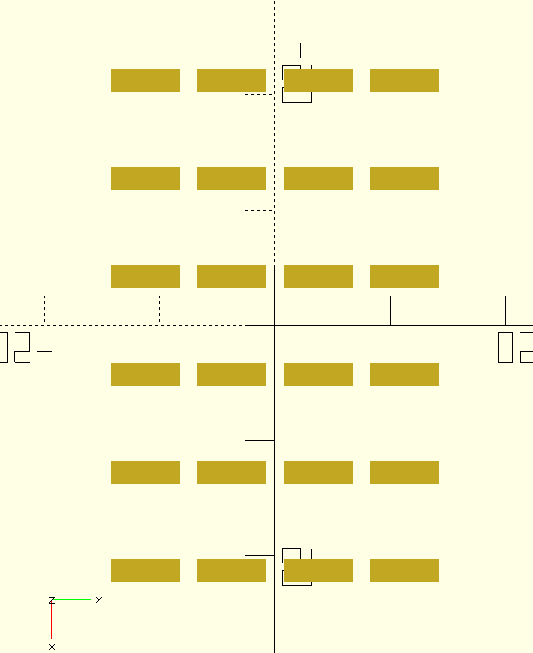
\includegraphics[width=.45\textwidth]{imagenes/matriz-completa-centrada-0}    
    \caption{Cecilia centra debidamente la matriz en el origen de
      coordenadas.}
    \label{fig:matriz-completa-centrada-0}
  \end{figure}
  


    Antonia aprobó la modificación con una sonrisa y un aplauso
    apagado: la traslación del arreglo ocurría gracias al
    \lstinline!translate! de las líneas 2 a 4, que afectaba a todo lo
    creado por el \lstinline!for! inmediato siguiente.

    Pero ahora fue Cecilia quien parecía mirar su propio texto con
    ojos críticos: las líneas 2 y 3 le parecieron demasiado similares
    a las 6 y 7. <<¿No estoy trasladando dos veces, y con una lógica
    similar, los mismos rayos de Sol?>> ---pensó---. <<¿Por qué no
    hacerlo de una sola vez..?>>. Y se lanzó a plasmar su idea:

\begin{lstlisting}
module digito(alfa){
  for(i=[0:5],j=[0:3]){
   x=(i-2.5)*(alto_pixel+delta_alto);
   y=(j-1.5)*(ancho_pixel+delta_ancho);
   translate([x,y,0])
    rayo_de_sol(alfa);
  } 
} 

digito(alfa=90);
    \end{lstlisting}


    % \begin{figure}[ht]
    %   \centering
    %   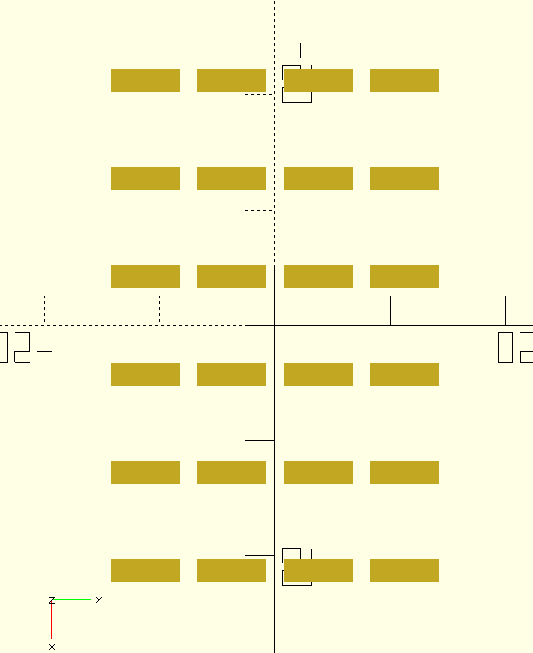
\includegraphics[width=.36\textwidth]{imagenes/matriz-completa-centrada-0}
    %   \caption{Cecilia pule su texto, transformando dos pares de
    %     traslaciones en uno solo.}
    %   \label{fig:matriz-completa-centrada-0-2}
    % \end{figure}


    
    ---Brillante, Cecilia, brillante...  ---Antonia quizá exageraba,
    pero a Cecilia no le importó: estaba muy orgullosa de su
    texto---. Esencialmente, sacaste factor común a las ecuaciones de
    las dos traslaciones.  Después de todo,
    $-2.5 \times (\text{alto\_pixel}+\text{delta\_alto})\, + \, i\times
    (\text{alto\_pixel}+\text{delta\_alto}) = (i-2.5) \times
    (\text{alto\_pixel}+\text{delta\_alto})$, y lo mismo vale para
    \coord{Y}.


    Cecilia creyó que ya podían dar por finalizado el capítulo, pero
    Antonia parecía querer alargarlo un poco más:

    ---Nos queda un detalle, que es mejor que resolvamos ahora. Como
    recordarás del capítulo \ref{semicilindro-1}, cuando restás un
    objeto de otro es conveniente que no compartan una cara en común,
    a fin de evitar una ambigüedad con respecto a la pertenencia o no
    de esa cara al objeto final. Y resulta que tus rayos de Sol se
    apoyan sobre el plano \coord{XY}, al igual que el semicilindro que
    deberán horadar:


\begin{lstlisting}
difference(){
  rotate([-90,0,0])
    semicilindro(150,30,center=true);  
  digito(alfa=90);
}
    \end{lstlisting}
%  \end{minipage}\hfill

    \begin{figure}[ht]
      \centering
      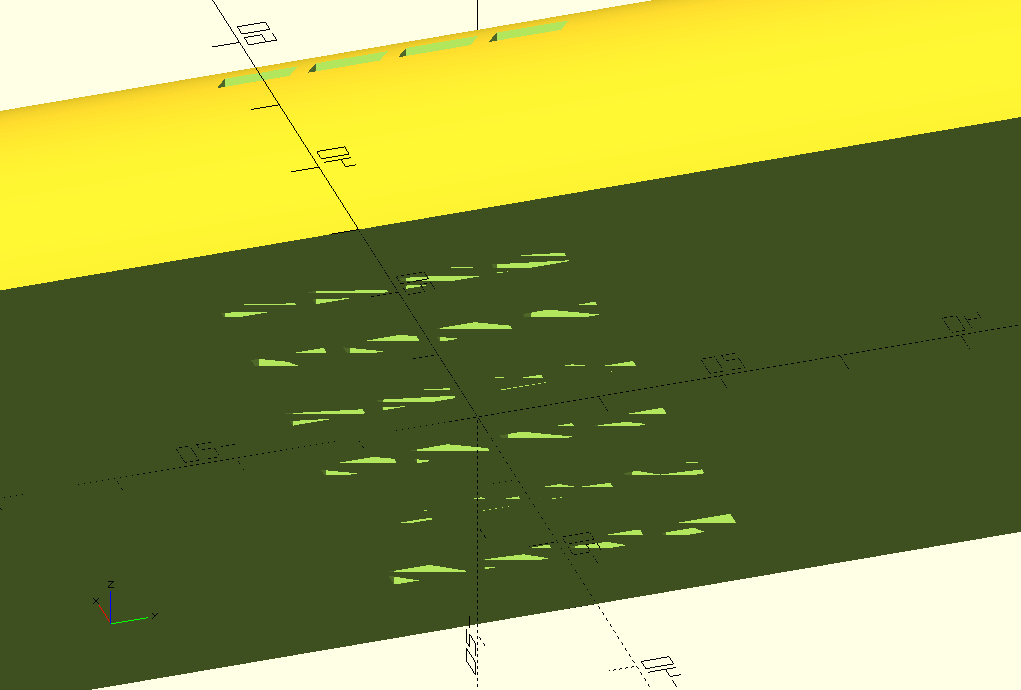
\includegraphics[width=.65\textwidth]{imagenes/digito-al-ras}
      \caption{Antonia muestra un \emph{bug} sutil del recientemente
        conquistado rayo de Sol.}
      \label{fig:digito-al-ras}
    \end{figure}
     



    ---Noooo.... ---gimió Cecilia, cubriendo sus ojos con una mano. La
    programación comenzó a dejar de parecerle divertida.

    ---Pero Cecilia... ¡no te vas a acorbardar por tan poco!
    ---Antonia la animó sin mucho tacto---. La hacemos fácil: bajamos
    cada rayo un toque. Muy poquito; apenas como para que la
    matemática de las diferencias de \openscad{} no se rompa:

    
\begin{lstlisting}
module digito(alfa){
  for(i=[0:5],j=[0:3]){
   x=(i-2.5)*(alto_pixel+delta_alto);
   y=(j-1.5)*(ancho_pixel+delta_ancho);
   translate([x,y,-0.01])
    rayo_de_sol(alfa);
  } 
}

difference(){
  rotate([-90,0,0])
    semicilindro(150,30,center=true);  
  digito(alfa=90);
}
    \end{lstlisting}
%  \end{minipage}\hfill

    \begin{figure}[ht]
      \centering
      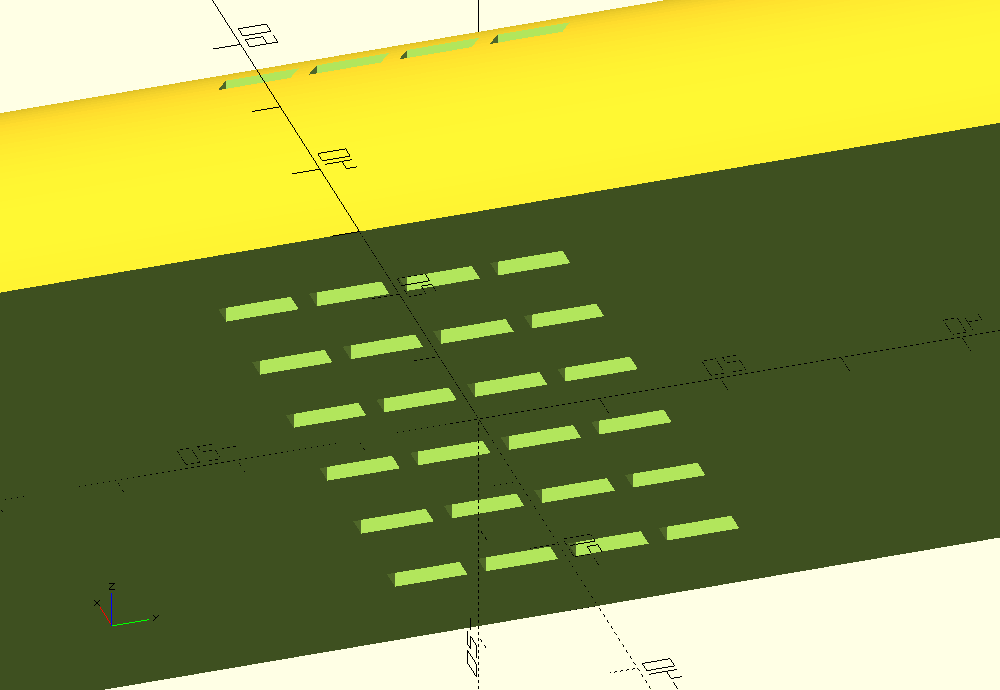
\includegraphics[width=.65\textwidth]{imagenes/digito-apenas-descendido}
      \caption{Antonia resuelve el \emph{bug} con un expediente
        sencillo pero eficaz.}
      \label{fig:digito-apenas-descendido}
    \end{figure}
      



    ---¿Ves? ---Antonia procuró parecer despreocupada, aunque tal vez
    sobreactuando un poco---. No se trata más que de trasladar cada
    rayo, en la línea 5, -0,01mm en el eje \coord{Z}...

    Cecilia podía apreciar en la figura
    \ref{fig:digito-apenas-descendido} que la solución de Antonia
    funcionaba, pero no estaba muy convencida:
    
    ---¿Y por qué 0,01?

    ---Pues... con que se trate de un valor negativo alcanza, y 0,01
    es mucho más bajo que la resolución de nuestra impresora 3D: en lo
    que respecta al objeto que produciremos, la diferencia con 0 es
    meramente formal ---Antonia trató de que su tono confiado
    pareciera un argumento. Cecilia juzgó que se trataba de una
    solución chapucera, pero no podía negar que funcionaba. Y la
    verdad es que ya estaba cansada.
    
    Pero antes de terminar quiso comprobar que nada se rompía usando
    otros ángulos, como 60º y 150º.



  \begin{figure}[ht]
    \centering
  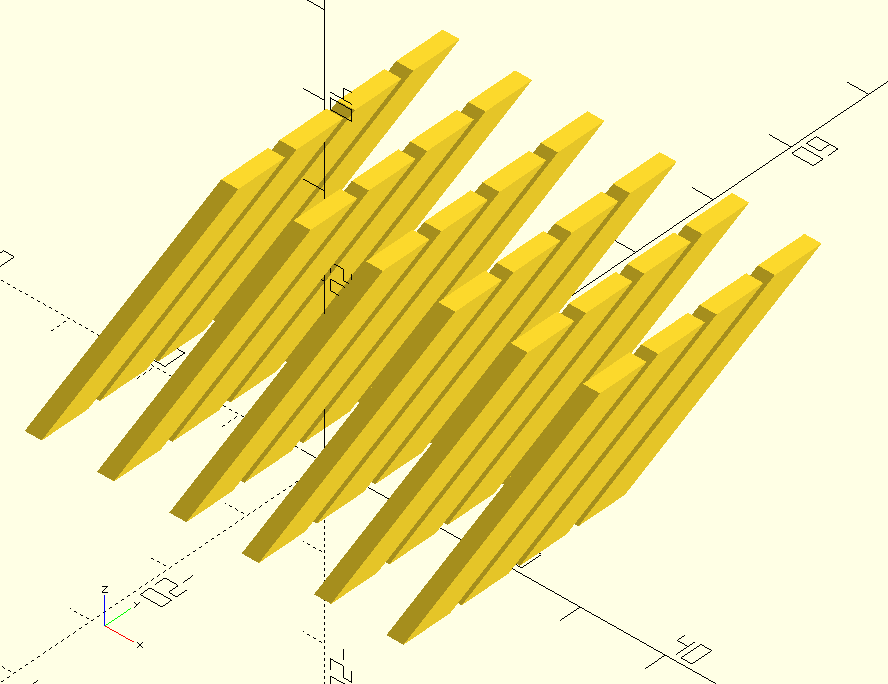
\includegraphics[width=.49\textwidth]{imagenes/matriz-60}\hfill
  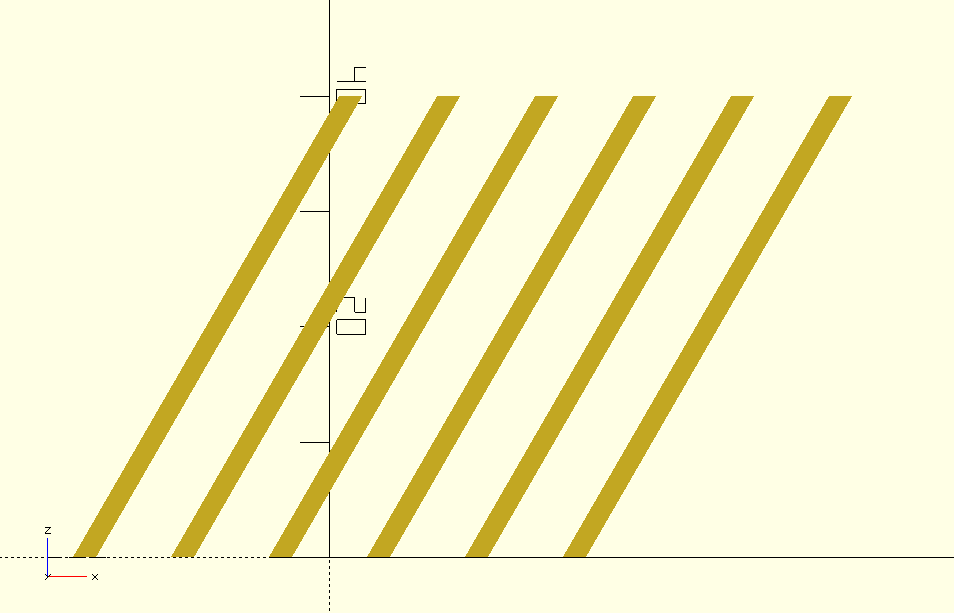
\includegraphics[width=.49\textwidth]{imagenes/matriz-60-perfil}
  \caption{Cecilia comprueba que el rayo de Sol funciona con 60º:
    \lstinline!digito(alfa=60);!...}
    \label{fig:matriz-60}
  \end{figure}
  

    \begin{figure}[h!]
    \centering
  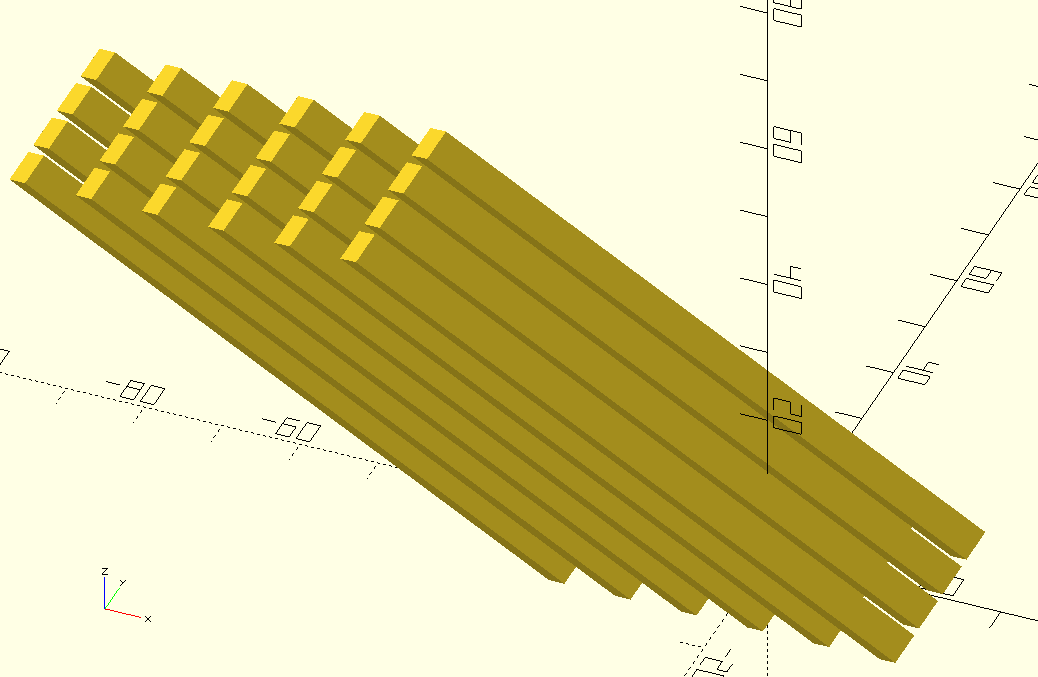
\includegraphics[width=.49\textwidth]{imagenes/matriz-150}\hfill
  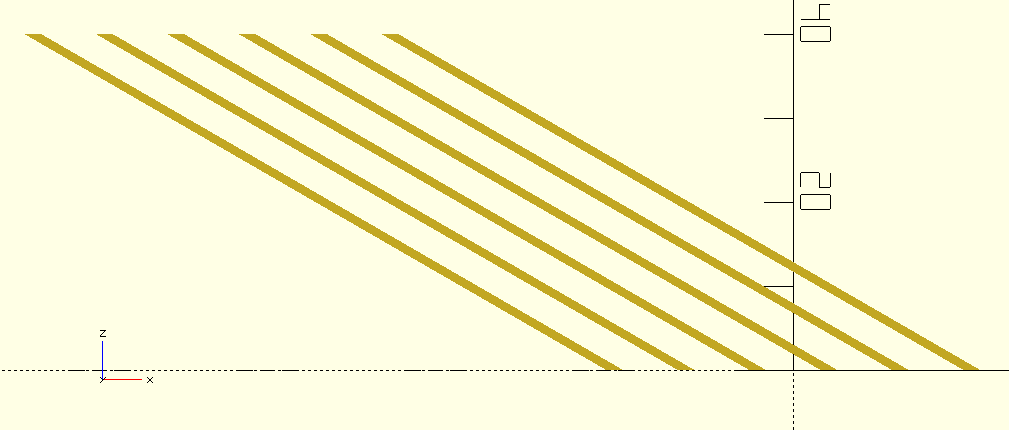
\includegraphics[width=.49\textwidth]{imagenes/matriz-150-perfil} 
    \caption{...y con 150º: \lstinline!digito(alfa=150);!}%\vspace{128in}
    \label{fig:matriz-150}
  \end{figure}

    Parecía que no.




%%% Local Variables:
%%% mode: latex
%%% TeX-master: "../libro"
%%% End:
